\section{【实现】可输出字符串的ucore}\label{ux5b9eux73b0ux53efux8f93ux51faux5b57ux7b26ux4e32ux7684ucore}

proj3包含了一个只能输出字符串的简单ucore操作系统,虽然简单,但它也体现了操作系统的一些结构和特征,比如它具有:

\begin{itemize}
\item
  完成给ucore的BSS段清零并显示一个字符串的内核初始化子系统(init.c)
\item
  提供串口/并口/CGA显示的驱动程序子系统(console.c)
\item
  提供公共服务的操作系统函数库子系统(printf.c printfmt.c string.c)
\end{itemize}

这体现了操作系统的一个基本特征:资源管理器。从操作系统原理我们可以知道一台计算机就是一组资源,这些资源用于对数据的移动、存储和处理并进行控制。在proj3中的ucore操作系统目前只提供了对串口/并口/CGA这三种I/O设备的硬件资源的访问,每个I/O设备的操作都有自己特有的指令集或控制信号(对照一下serial\_putc/lpt\_putc/cga\_putc函数的实现),操作系统隐藏这些细节,并提供了统一的接口(看看cprintf函数的实现),因此程序员可以使用简单的printf函数来写这些设备,达到显示数据的效果。目前操作系统的逻辑结构图架构如下图所示:

\begin{figure}[htbp]
\centering
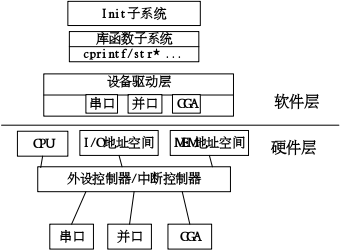
\includegraphics{figures/3.2.7.1.png}
\caption{3.2.7.1}
\end{figure}

在PC中的地址空间布局图如下所示:

\begin{figure}[htbp]
\centering
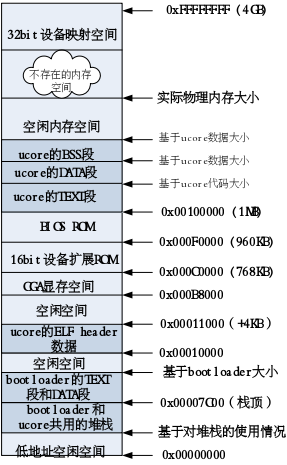
\includegraphics{figures/3.2.7.2.png}
\caption{3.2.7.2}
\end{figure}
